\documentclass[border=10pt]{standalone}
\usepackage{pgfplots}
\pgfplotsset{compat=1.18}
\usepackage{tikz}

\begin{document}
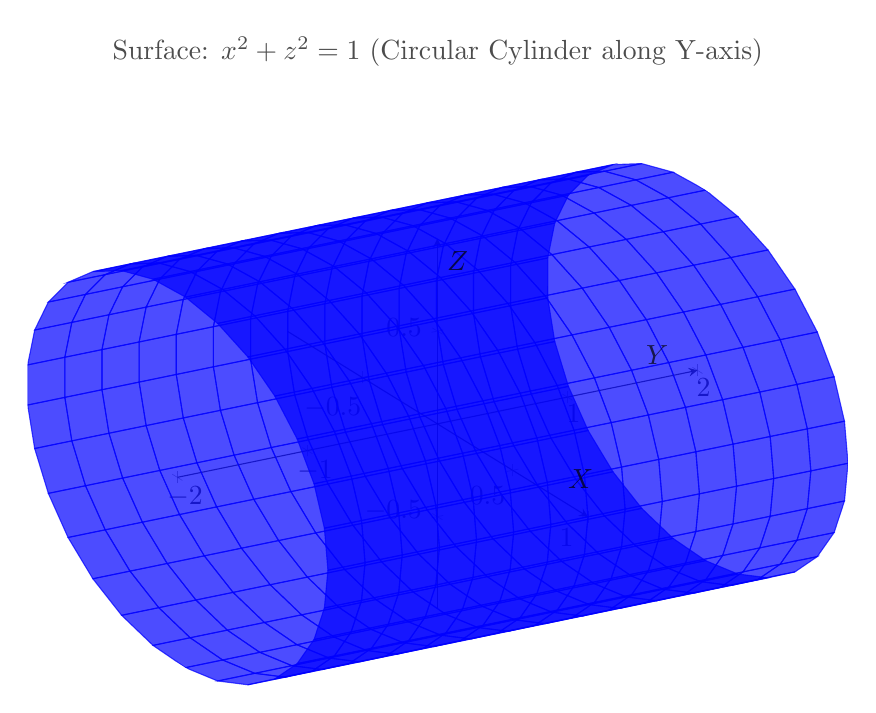
\begin{tikzpicture}
\begin{axis}[
    width=12cm,
    height=10cm,
    view={60}{30},
    xlabel=$X$,
    ylabel=$Y$,
    zlabel=$Z$,
    title={Surface: $x^2 + z^2 = 1$ (Circular Cylinder along Y-axis)},
    axis lines=center,
    grid=major,
    domain=0:360,
    y domain=-2:2,
    samples=30,
    samples y=15,
    z buffer=sort,
    opacity=0.7,
]
    \addplot3[surf, blue, shader=flat] ({cos(x)}, {y}, {sin(x)});
\end{axis}
\end{tikzpicture}
\end{document}